\subsection{研究報告(松島)}
本節では松島研究室の研究活動について報告する。
2019年度および2020年度に、弊研究室では解釈可能な機械学習手法の効率的な計算手法についての研究を推進してきた。

画像データや言語データを予測したり生成したり表層的に駆使することは可能になってきた。
しかしながら我々の画像や言語の理解が進んだわけではない。

機械学習は予測や分類など表層的なデータの駆使の方法論であるだけでなく、
データの関係を明らかにして人間の理解を助けるための方法論でもある。

特にデータ保持者の目線に立って機械学習を


成果は主に以下の3分野に大別される。
\begin{itemize}
    \item 一般化加法モデルに関する研究
    \item 組合せ線形モデルに関する研究
    \item 部分空間クラスタリングに関する研究
\end{itemize}

一般化加法モデルと組み合わせ線形モデルは
属性間の線形な関係を越えて、非線形な関係を抽出するための枠組みである。
部分空間クラスタリングはデータ集合が持つ単純な線形関係を超えて、
データのクラスタリングを行ってそれぞれのクラスタが持つ線形関係を抽出する枠組みである。


\subsubsection{一般化加法モデルに関する研究}
いわゆる線形モデルの学習とは以下のようにあらわされる
データの属性間の線形な関係を抽出する枠組みととらえることができる
\begin{align*}
    y = \sum_{j} w_j x_j
\end{align*}
データの属性$y$は通常予測したい変数であり、
他のデータ属性が$x_j$である。与えられたデータ集合を用いて$w_j$は実数全体から推定される。
一般化加法モデルでは以下のような関係を抽出する枠組みである
\begin{align*}
    y = \sum_{j} f_j (x_j)
\end{align*}
与えられたデータ集合を用いて$f_j$は(十分広い)関数クラス$F$から推定される。
このような$f_j$を推定できれば、例えば年齢と収入の非線形な関係などがデータから
学習できると考えられる。

最も単純な手法は$F$を推定の簡単さのために狭めの関数クラスに制限することである。
一般に与えられた基底関数集合$\left\{\varphi_k(\cdot):\mathbb{R} \to \mathbb{R} \right\}_{k=1,\ldots,K}$に対し
\begin{align*}
  F=\left\{  \sum_{k=1}^d \varphi_k(x_j) \right\}
\end{align*}
とすることはパラメトリックな手法と呼ばれる。
\cite{F}は〜\\

利用可能なデータ数に応じて関数クラスの大きさが変わる。
具体的にはデータ数が大きくなれば関数クラスも広くなっていくような手法をノンパラメトリックな手法と呼び、
そのような手法はカーネル法を使うよりなかった。
我々の手法はカーネル法よりも効率的に学習が可能である。


さらに複雑な関係性をデータから学習して可視化することが可能である
\begin{align*}
    y = \sum_{j,k} f_{j,k} (x_j,x_k)
\end{align*}




\subsubsection{組合せ線形モデルに関する研究}

組合せ線形モデルでは離散データ集合を考える。
離散データも多くの現実のデータを表現することができる。

組合せ線形モデルは回帰やクラス分類などの教師あり学習の手法のためのモデルであり、各説明変数の論理結合を特徴として線形関数を学習する手法である\cite{LMY01}。論理結合による特徴は各説明変数が同時に真である場合の効果を表すと解釈できるため、解釈性も予測性能も高い予測が可能である(図1参照)。
本研究では、論理結合による特徴を膨大な候補集合から探索する際に高速な頻出パターンマイニングのアルゴリズムを利用するなどのアプローチにより、組み合わせ線形モデルの学習アルゴリズムの改良を行う。

さらに高次対数線形モデルと呼ばれる組み合わせ線形モデルの生成モデルの研究を行った。
高次対数線形モデルは
\begin{align*}
    \log P(x;\theta) = \sum_{\phi\in B} \theta_\phi \phi(x)  - \log\left( \sum_{x'\in S} \exp\left( \sum_{\phi\in B} \theta_\phi \phi(x') \right) \right)    
\end{align*}
ここで$\phi \in B \subset \{0,1\}^n$と$\phi:\{0,1\}^n\to \{0,1\} $を同一視する。すなわち$\phi(x)$の値を以下で定義する。
\begin{align*}
    \phi(x)  = \begin{cases}
    1 & 全ての j で \phi_j \le x_j, \\
    0 & 上記以外.
    \end{cases}
\end{align*}

さらに二値データの分布の推定問題を考える。
NSという概念を導入し、よりNSが高いモデルを推定するような定式化と方法論を提案する。


\subsubsection{部分空間クラスタリングに関する研究}

部分空間クラスタリングとは複数の低次元空間にデータをクラスタリングする手法である。通常のクラスタリング手法では距離的に近いデータの集まりをクラスタとみなす。一方で、部分空間クラスタリングでは同じ低次元空間にあるデータをクラスタとみなす(図1を参照)。画像データや文章データなどはタスクによって部分空間クラスタリングをした方がよいということが2011年VIDAL\cite{SC}によって提案されて以降、多くの部分空間クラスタリング手法が開発されている。

\begin{figure}[h]
    \centering
    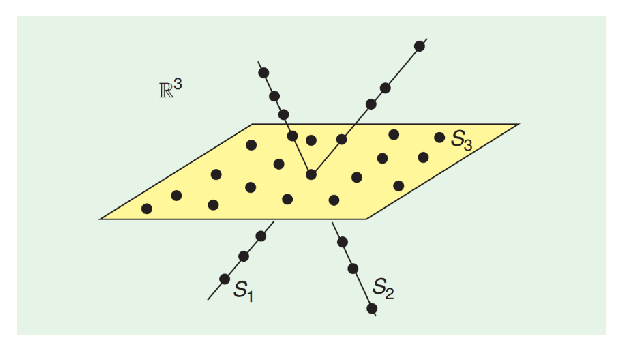
\includegraphics[width=7cm]{Matsushima/sc.eps}
    \caption{部分空間クラスタリングの3次元の例(\cite{SC}から抜粋)。距離が近い点同士ではなく、同じ平面上もしくは同じ直線上(部分空間上)にある点同士をクラスタとみなす。}
    \label{fig:my_label}
\end{figure}
\cite{HSM01}は〜\\
\cite{HSM02}は〜\\
\cite{KM01}は〜\\
\cite{KM02}は〜\\
\cite{NM01}は〜

\begin{thebibliography}{9}
\bibitem{F}
    Friedman, J., Hastie, T., & Tibshirani, R. (2010). 
    Applications of the lasso and grouped lasso to the estimation of sparse graphical models (pp. 1-22). Technical report, Stanford University.
\bibitem{SC}
 VIDAL, René. Subspace clustering. IEEE Signal Processing Magazine, 2011, 28.2: 52-68.
\end{thebibliography}

